\chapter{Evaluation}

\section{Customer Requirements}

These are the original objectives specified by the client at the analysis stage of making this system.

\textbf{General Objectives}

\begin{itemize}
	\item To have an interactive and easily navigable graphical user interface, applying a suitable colour scheme and layout
	\item To make the database concise and adjustable
	\item To create various lessons, with a wide range of challenges, which effectively teach students how to do trigonometry and Pythagoras
	\item To create tasks which are relevant to the lessons to be completed by the user in order to test their progress
	\item To allow this progress to be recorded in an easily accessible and readable database
	\item To incorporate algorithms which find and/or check the solution given by the user accurately and give clear and easy to read outputs to correspond with said inputs
	\item To have some access restrictions to certain levels of user
	\item To make the program accessible only from various computers with permissions
\end{itemize}

\textbf{Specific Objectives}

\begin{itemize}
	\item To create a teaching program that uses the new GCSE Maths curriculum, as lots of resources will soon be out of date
	\item To include the following topics: Trigonometry, Pythagoras, 3D Trigonometry, 3D Pythagoras
	\item To include a range of difficulty levels, which can challenge every user's level of ability
	\item Use drag and drop, text boxes and drop down menus for inputs
	\item To include interactive 2D graphics which give a clearer idea of the method being shown to the user
	\item To have a database which can be accessed by different computers online
	\item Use a specific, continuous and attractive colour scheme in every window
	\item To have medium sized, highly visible icons
	\item To have all input buttons randomised to avoid double clicking and guessing from memory
	\item To have small error message windows which pop up and disappear on a timer
	\item To include images and shapes which contrast the colour scheme so they are visible and readable
\end{itemize}

\textbf{Core Objectives}

\begin{itemize}
	\item To create a teaching program that uses the new GCSE Maths curriculum, as lots of resources will soon be out of date
	\item To make the database easy to access and easy to read
	\item To include primarily trigonometry based topics, such as how to use the sine, cosine and tan rules
	\item To include an initial, moderate difficulty in order to cater for a majority of students
	\item To make the database functional and able to store the requested details
\end{itemize}

\textbf{Other Objectives}

\begin{itemize}
	\item To position buttons, text boxes and drag and drop boxes in within the layout of the graphical user interface in such a way that cheating and lucky guessing can be minimised
	\item To make the database adjustable if necessary
	\item Use a more interesting range of input types like drawing boxes rather than just clicking and typing
	\item To include a wider range of difficulties to challenge every student on the right level for them
	\item To include a wider range of topics such as pythagoras, then 3D trigonometry and 3D pythagoras
\end{itemize}

\subsection{Objective: }

To have an interactive and easily navigable graphical user interface, applying a suitable colour scheme and layout

\subsubsection{Objective Met?}

Yes/no 

\subsubsection{Evidence: }

Evidence

\subsection{Objective: }

To make the database concise and adjustable

\subsubsection{Objective Met?}

Yes/no 

\subsubsection{Evidence: }

Evidence

\subsection{Objective: }

To create various lessons, with a wide range of challenges, which effectively teach students how to do trigonometry and Pythagoras

\subsubsection{Objective Met?}

Yes/no 

\subsubsection{Evidence: }

Evidence

\subsection{Objective: }

To create tasks which are relevant to the lessons to be completed by the user in order to test their progress

\subsubsection{Objective Met?}

Yes/no 

\subsubsection{Evidence: }

Evidence

\subsection{Objective: }

To allow this progress to be recorded in an easily accessible and readable database

\subsubsection{Objective Met?}

Yes/no 

\subsubsection{Evidence: }

Evidence

\subsection{Objective: }

To incorporate algorithms which find and/or check the solution given by the user accurately and give clear and easy to read outputs to correspond with said inputs

\subsubsection{Objective Met?}

Yes/no 

\subsubsection{Evidence: }

Evidence

\subsection{Objective: }

To have some access restrictions to certain levels of user

\subsubsection{Objective Met?}

Yes/no 

\subsubsection{Evidence: }

Evidence

\subsection{Objective: }

To make the program accessible only from various computers with permissions

\subsubsection{Objective Met?}

Yes/no 

\subsubsection{Evidence: }

Evidence

\subsection{Objective: }

To create a teaching program that uses the new GCSE Maths curriculum, as lots of resources will soon be out of date

\subsubsection{Objective Met?}

Yes/no 

\subsubsection{Evidence: }

Evidence

\subsection{Objective: }

To include the following topics: Trigonometry, Pythagoras, 3D Trigonometry, 3D Pythagoras

\subsubsection{Objective Met?}

Yes/no 

\subsubsection{Evidence: }

Evidence

\subsection{Objective: }

To include a range of difficulty levels, which can challenge every user's level of ability

\subsubsection{Objective Met?}

Yes/no 

\subsubsection{Evidence: }

Evidence

\subsection{Objective: }

Use drag and drop, text boxes and drop down menus for inputs

\subsubsection{Objective Met?}

Yes/no 

\subsubsection{Evidence: }

Evidence

\subsection{Objective: }

To include interactive 2D graphics which give a clearer idea of the method being shown to the user

\subsubsection{Objective Met?}

Yes/no 

\subsubsection{Evidence: }

Evidence

\subsection{Objective: }

To have a database which can be accessed by different computers online

\subsubsection{Objective Met?}

Yes/no 

\subsubsection{Evidence: }

Evidence

\subsection{Objective: }

Use a specific, continuous and attractive colour scheme in every window

\subsubsection{Objective Met?}

Yes/no 

\subsubsection{Evidence: }

Evidence

\subsection{Objective: }

To have medium sized, highly visible icons

\subsubsection{Objective Met?}

Yes/no 

\subsubsection{Evidence: }

Evidence

\subsection{Objective: }

To have all input buttons randomised to avoid double clicking and guessing from memory

\subsubsection{Objective Met?}

Yes/no 

\subsubsection{Evidence: }

Evidence

\subsection{Objective: }

To have small error message windows which pop up and disappear on a timer

\subsubsection{Objective Met?}

Yes/no 

\subsubsection{Evidence: }

Evidence

\subsection{Objective: }

To include images and shapes which contrast the colour scheme so they are visible and readable

\subsubsection{Objective Met?}

Yes/no 

\subsubsection{Evidence: }

Evidence

\subsection{Objective: }

To create a teaching program that uses the new GCSE Maths curriculum, as lots of resources will soon be out of date

\subsubsection{Objective Met?}

Yes/no 

\subsubsection{Evidence: }

Evidence

\subsection{Objective: }

To make the database easy to access and easy to read

\subsubsection{Objective Met?}

Yes/no 

\subsubsection{Evidence: }

Evidence

\subsection{Objective: }

To include primarily trigonometry based topics, such as how to use the sine, cosine and tan rules

\subsubsection{Objective Met?}

Yes/no 

\subsubsection{Evidence: }

Evidence

\subsection{Objective: }

To include an initial, moderate difficulty in order to cater for a majority of students

\subsubsection{Objective Met?}

Yes/no 

\subsubsection{Evidence: }

Evidence

\subsection{Objective: }

To make the database functional and able to store the requested details

\subsubsection{Objective Met?}

Yes/no 

\subsubsection{Evidence: }

Evidence

\subsection{Objective: }

To position buttons, text boxes and drag and drop boxes in within the layout of the graphical user interface in such a way that cheating and lucky guessing can be minimised

\subsubsection{Objective Met?}

Yes/no 

\subsubsection{Evidence: }

Evidence

\subsection{Objective: }

To make the database adjustable if necessary

\subsubsection{Objective Met?}

Yes/no 

\subsubsection{Evidence: }

Evidence

\subsection{Objective: }

Use a more interesting range of input types like drawing boxes rather than just clicking and typing

\subsubsection{Objective Met?}

Yes/no 

\subsubsection{Evidence: }

Evidence

\subsection{Objective: }

To include a wider range of difficulties to challenge every student on the right level for them

\subsubsection{Objective Met?}

Yes/no 

\subsubsection{Evidence: }

Evidence

\subsection{Objective: }

To include a wider range of topics such as pythagoras, then 3D trigonometry and 3D pythagoras

\subsubsection{Objective Met?}

Yes/no 

\subsubsection{Evidence: }

Evidence
















 
\section{Effectiveness}

%include as many subsections as necessary for your objectives
\subsection{Objective Evaluation}






\section{Learnability}

When I first consulted my client I took into account how much experience they have already had using software such as my system. They are comfortable using the internet, so with the assistance of the user manual they should have no problem installing Python 3.4 and PyQt4. They, along with the other people the client intends to use this system with, have all had experience using similar educational maths programs, such as MyMaths, which have essentially the same purpose as my system. Therefore I tried to make some aspects of the system somewhat similar to the ones conventionally used in educational maths programs, such as the layout, including the navigation of the system, the topics, and the rules of saving and popping error messages, such as making sure all questions have been attempted. None the less, this system would probably be easy enough for less experienced users anyway, as generally the buttons are clearly labelled, appropriately sized, and organised in a convenient way (branch menu). Although some users may have issues finding the exact right topic in the sub-menus, being a reason for the big red return buttons which make it easy to go back and try another menu.

\begin{figure}[H]
	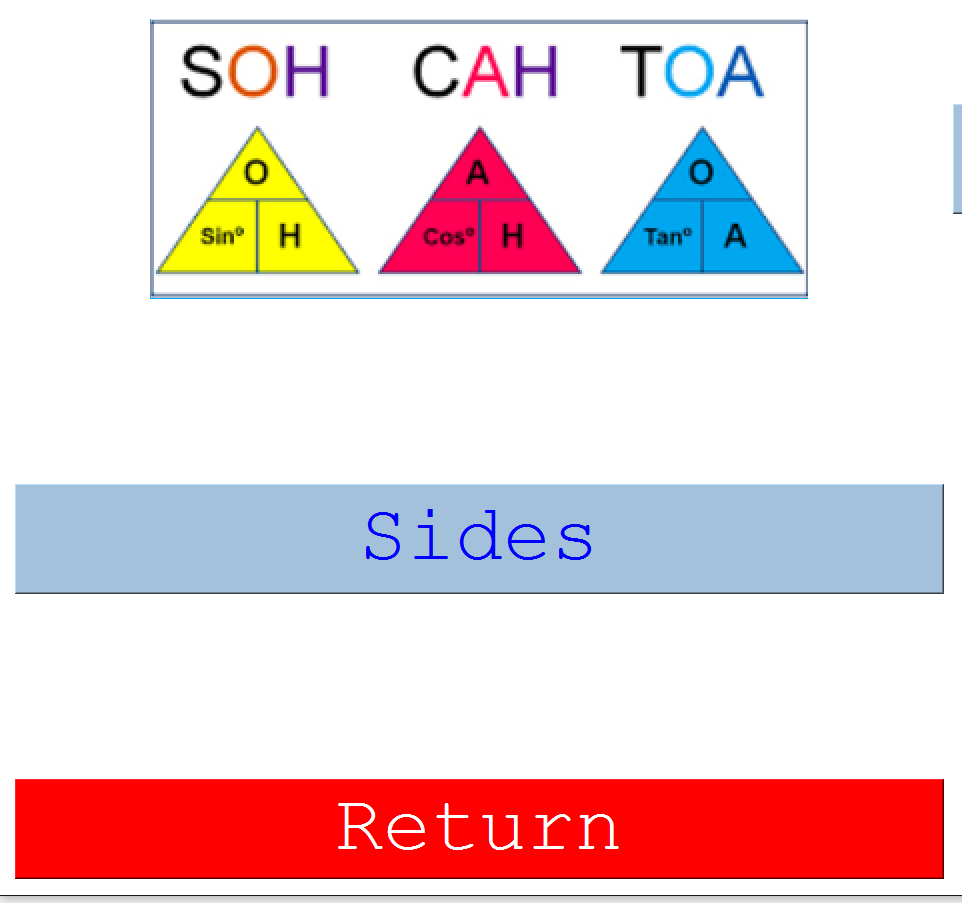
\includegraphics{C:/Users/Jordan/git/COMP4Coursework2/Evaluation/learnability_1}
	\caption{An example of the return buttons used to make navigating the sub-menus easier}
\end{figure}

When designing the system I kept in mind the fact that saving data can be a more complex function if it is done manually, especially by an inexperienced user, so I made all of the database functions automatic; they occur when the user simply clicks a button to finish a homework, or opens the progress screen. This cancels out the need for users to learn new skills which they might not have already learned from using similar systems.

\begin{figure}[H]
	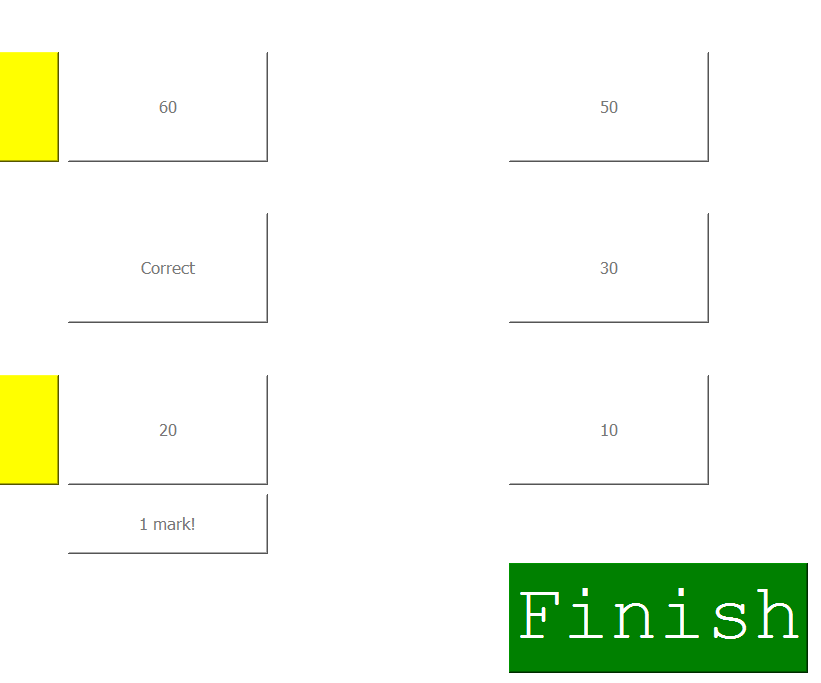
\includegraphics{C:/Users/Jordan/git/COMP4Coursework2/Evaluation/learnability_2}
	\caption{The finish button being clicked to automatically save progress for the user}
\end{figure}

\begin{figure}[H]
	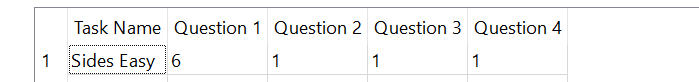
\includegraphics{C:/Users/Jordan/git/COMP4Coursework2/Evaluation/learnability_3}
	\caption{The record which was just saved immediately being updated to the database}
\end{figure}

I also endeavoured to make the database itself very easy to access and understand internally in the system; the system accesses the information from a separate file and displays it in a window in the program, which can be accessed by the user very quickly from the home screen, and even queried for specific details should the user be searching for a specific record. the options in hte combo boxes are as clear as I can make them to make it easier for the user to determine how to use the query function when they try it for the first time.

\begin{figure}[H]
	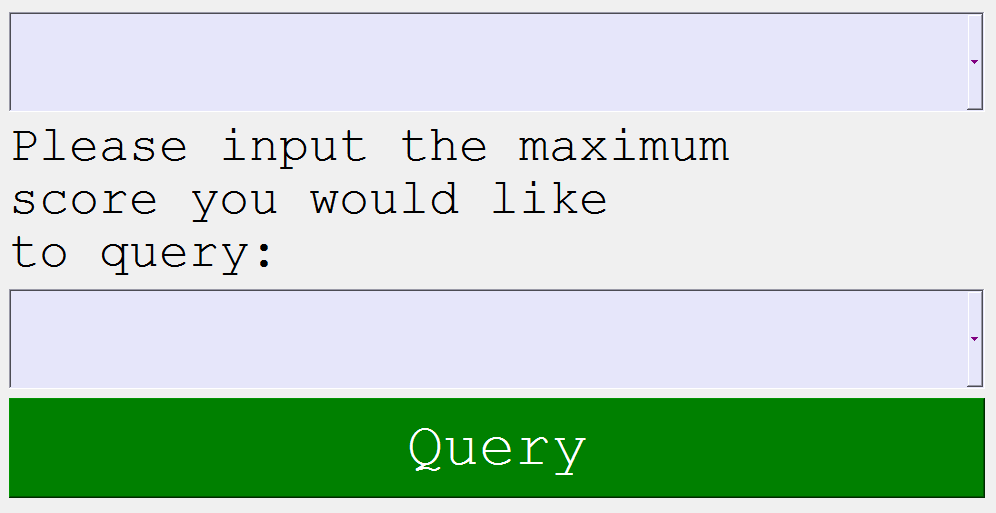
\includegraphics{C:/Users/Jordan/git/COMP4Coursework2/Evaluation/learnability_4}
	\caption{An example of the database being queried for easy access to specific records}
\end{figure}

Error messages were also incorporated to help the user understand why the sytem isn't working as they expected, should they fail to answer a question properly and try to proceed to the next page and be unsure why they cannot.

\begin{figure}[H]
	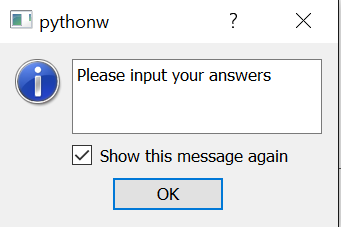
\includegraphics{C:/Users/Jordan/git/COMP4Coursework2/Evaluation/learnability_5}
	\caption{An example of an error message telling the user why they cannot proceed}
\end{figure}

Generally, this system is very easy to use, even for people with little experience with such software, and care has been taken to ensure that the interface is very clear and the error messages are sufficient to help a user fix a progression related problem should they need the help. The only concern is that the user has no way to reset the database internally, so once they start using the system they have to either keep their progress or delete the database file manually.

\section{Usability}

I shall evaluate how easy to use each different aspect of the system is in order to gain an idea of whether or not the overall system has a good level of usability. The criteria I will use to measure the usability of each aspect include readability, convenience, time spent looking across the screen for things and common logic which the user needs to be able to understand.

The graphical user interface has large buttons with clear, blunt text which states the purpose of the button. The buttons also have a user friendly colour scheme which helps to make it clear what might happen when a button is clicked. For example, yellow means to mark an input, blue means to continue to a new screen, and red means to return to a previous screen. This assists the user in distinguishing the purposes of buttons which are sometimes positioned quite close to each other. The sub menus have six buttons, five which open a new menu and one which returns to a past screen, so it helps the user to immediately see which of the six buttons is going to take them back. The user expressed a high level of satisfaction with the user interface in general, suggesting that already it is a very usable interface. All of the input boxes have been sized to match the buttons, and the pictures have been sized to fit in the left over spaces, and to be relevant to the buttons they are placed next to, such as a trigonometry picture next to the trigonometry menu button. The readability of the graphical user interface is good, as all of the text has been enlarged to fill the screen as appropriate, so a user should have no trouble figuring out which buttons to click to find things in the system. The database screen and report widgets are accessible after three mouse clicks, and each lesson or homework after five, so it is convenient to get to any screen if you know where it is. The downside is perhaps having to search through each sub menu to find a topic. All of the widgets are pretty much equally sized, so target acquisition for the users eyes should be fast all round. Finally, each button is labelled appropriately, each picture is relevant and each title is clear, so there is common logic for the user to understand easily when navigating the system. Overall, the graphical user interface has a high usability level.

\begin{figure}[H]
	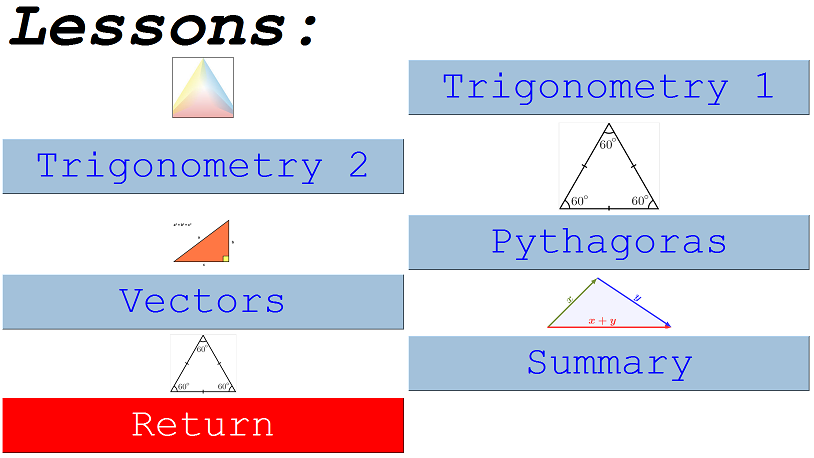
\includegraphics{C:/Users/Jordan/git/COMP4Coursework2/Evaluation/usability_1}
	\caption{An example of the highly readable and easy to navigate menus}
\end{figure}

The storage of data has, in some ways, a high level of usability, but a low level in others. Firstly, it has a high level of usability because the user literally does not have to do any manual saving, loading, or database management, as the system saves and reads everything internally and automatically at certain points. All they need to do is complete the homeworks using easy inputs and maths skills, the learning of which is their responsibility, in order to record progress. They do not need to learn any new skills to be able to maintain the system's records, which can be considered convenient, should the user wish to stick to one 'attempt' at getting the best scores they can from the sytem. However, if the user wanted to delete their current progress and start again, they would have to manually remove the database file in order to reset their progress, which they might not know how to do. the lack of an internal 'drop table' function could be seen as inconvenient, despite it not being the purpose of the system or a client specified objective. Furthermore, the system does not save all of the data which the client wanted to be saved; only about half of the objective information is recorded throughout the system. Therefore the entire database itself has limited usability as the client will struggle to keep track of student's progress as originally intended. The information itself is all displayed in a table widget on the progress screen two clicks away from the welcome screen, so is quick to access and find as it is displayed in a huge table in the top right corner of the screen, one of the places where the user is likely to look first. The text itself is a nice size and is on a well-contraasted white background. In order to improve convenience, time spent and common logic I implemented a report widget where the user can quickly and easily query the database using large and easily usable combo boxes to select query criteria, the results of which will then appear in a similar table widget for the user to view immediately. Overall, the level of usability of the database is moderate, as information can be easily and quickly viewed, and recorded without any extra skills from the user, however once they start using the system they have to stick with the database they have unless they manually delete it.

\begin{figure}[H]
	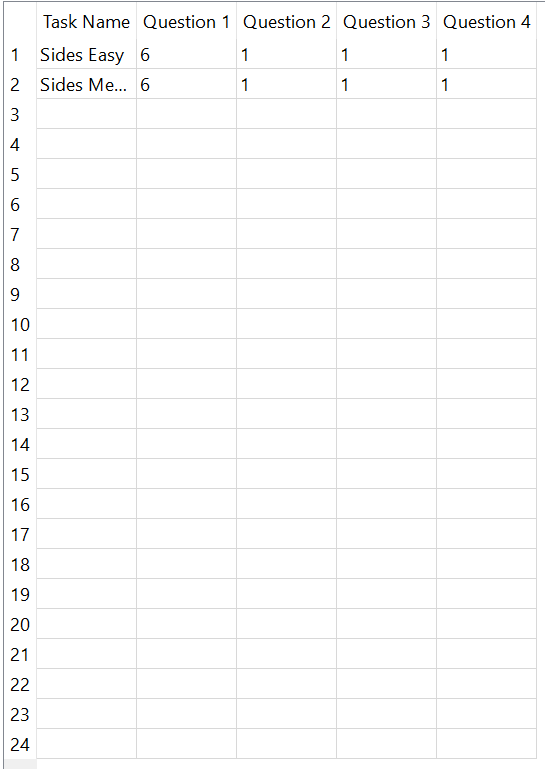
\includegraphics{C:/Users/Jordan/git/COMP4Coursework2/Evaluation/usability_2}
	\caption{Shows the clearly displayed information from the database}
\end{figure}

The subject material used in this system's lessons and homework sections is built up using large, clear text in a readable font against a nicely contrasting background color, accompanied by relevant pictures which can also show the user a mathematical method graphically, and large, clearly purposed buttons, line edits and combo boxes for a variation of input types. The user should have no trouble understanding what the questions are asking of them, and the lessons are supported by sufficient graphical images and text to give the user a clear example of a mathematical technique used to solve a problem. All of the images have either a good or a reasonable resolution. The buttons make it clear how to proceed or return to a previous screen. The colours used are all kind on the eyes. At no point should the user spend more than twenty seconds navigating from screen A to screen B (e.g. welcome screen to a homework screen) as the menus are all easy to use and understand. Therefore, generally the physical appearance of the system gives it quite a high usability.

\begin{figure}[H]
	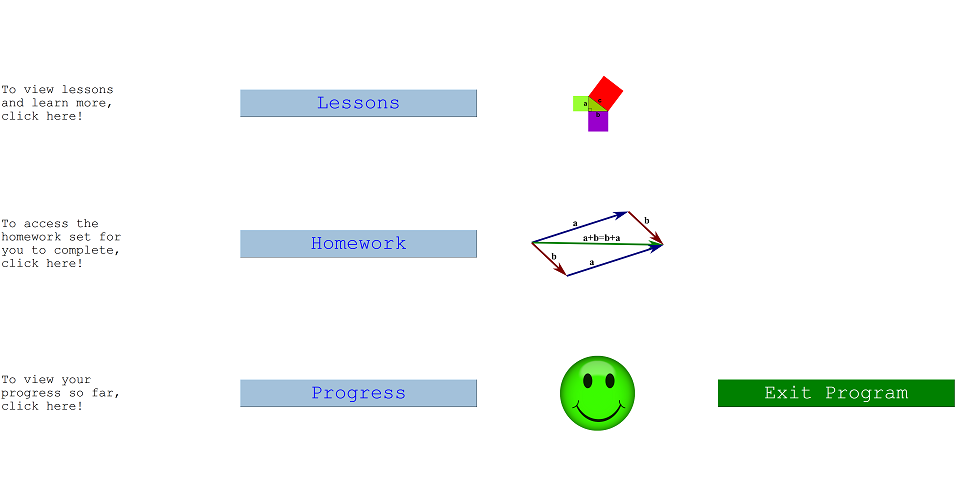
\includegraphics{C:/Users/Jordan/git/COMP4Coursework2/Evaluation/usability_3}
	\caption{The home screen showing the good colour scheme and the high resolution pictures}
\end{figure}

The error messages used in the system have a sole purpose of making it easier for hte user to use, therefore they naturally have a high level of usability. I have ensured that they are easy to understand and dismiss, and only appear when absolutely necessary to minimise disturbance for the user. The only foreseeable potential issue with the error messages is that they are quite small, so the user might have to squint to properly read the text, depending on the size of their monitor and the distance between their eyes and the screen. Otherwise, the text is simple and make it obvious what the problem is (all of the problems which might trigger errors in the system at all are simple ones), and they are dismissable by simply clicking the 'ok' button in the middle. Readibility is limited, convenience is high, as they only appear to help the user, time spent looking is low as they appear right in the middle of the screen making them impossible to miss, and common logic is high as they give clear instructions to the user. Therefore the only thing limiting the error messages' usability slightly is their small size, which is a result of using default QErrorMessage widgets. Otherwise error message usability is overall a high level.

\begin{figure}[H]
	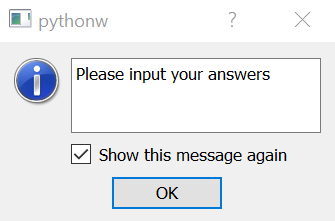
\includegraphics{C:/Users/Jordan/git/COMP4Coursework2/Evaluation/usability_4}
	\caption{An example of the small but clear error messages}
\end{figure}

Conclusively, the usability level of the overall system is reasonably high, as three of the four aspects of the system have been measured to have a high level of usability, and only one has a low-level of usability.

\section{Maintainability}

My system should be very easy to maintain. As of the completion of version 1 of the system, there are no bugs or errors which flag up in the IDLE, and there are no infinite loops or dead ends which the user wouldn't be able to escape without closing the entire application and restarting it. So unless more entire modules were added in a future version, there are currently no bugs to be maintained or fixed. I have used clear variable names throughout the modules which make it somewhat obvious what their purposes are, such as \textbf{self.layout} consistently for the PyQt4 layout of each window. Generic names have been used where required for each type of variable, such as \textbf{count} for stepper variables. Because I have so many sub classes within my system, I was able to use similar names for each sub class, such as \textbf{Trig1StackSidesEasy} and \textbf{Trig1StackSidesMedium} where classes inherit from the same parent class. For every parent class, all of its subclasses are created and altered in the same file; all of the first lesson page classes are in the same file, with almost exactly the same layout, and all of the second lesson pages are in a different file together, also with almost the same layout. This way, a programmer can determine what type of window the error is occurring on, look at the title of the window, and find the subclass easily in the file with the subclasses for that type of window. All of my code has been formatted in such a way that makes it easier to find bits of code. For example, the class begins at the top, followed by a constructor and the super(), then all of the PyQt variables are assigned, followed by algorithm variables, then PyQt window structuring, then connections, and lastly the methods in the order of the buttons they were connected to (this system is almost entirely event-driven). Furthermore, all of the database controller code is in one clearly named file, so if there are any problems involving the modification or accessing of the database the programmer will know where to look. Finally, every different line of code has been commented on at least once (some code is used consistently in many files, so an explanation will be in at least one of them). These comments give a clear explanation of the code's purpose and how it works or what it connects to. Therefore, a programmer will be able to find which section of code is responsible for causing a problem by reading the comments.

\begin{figure}[H]
	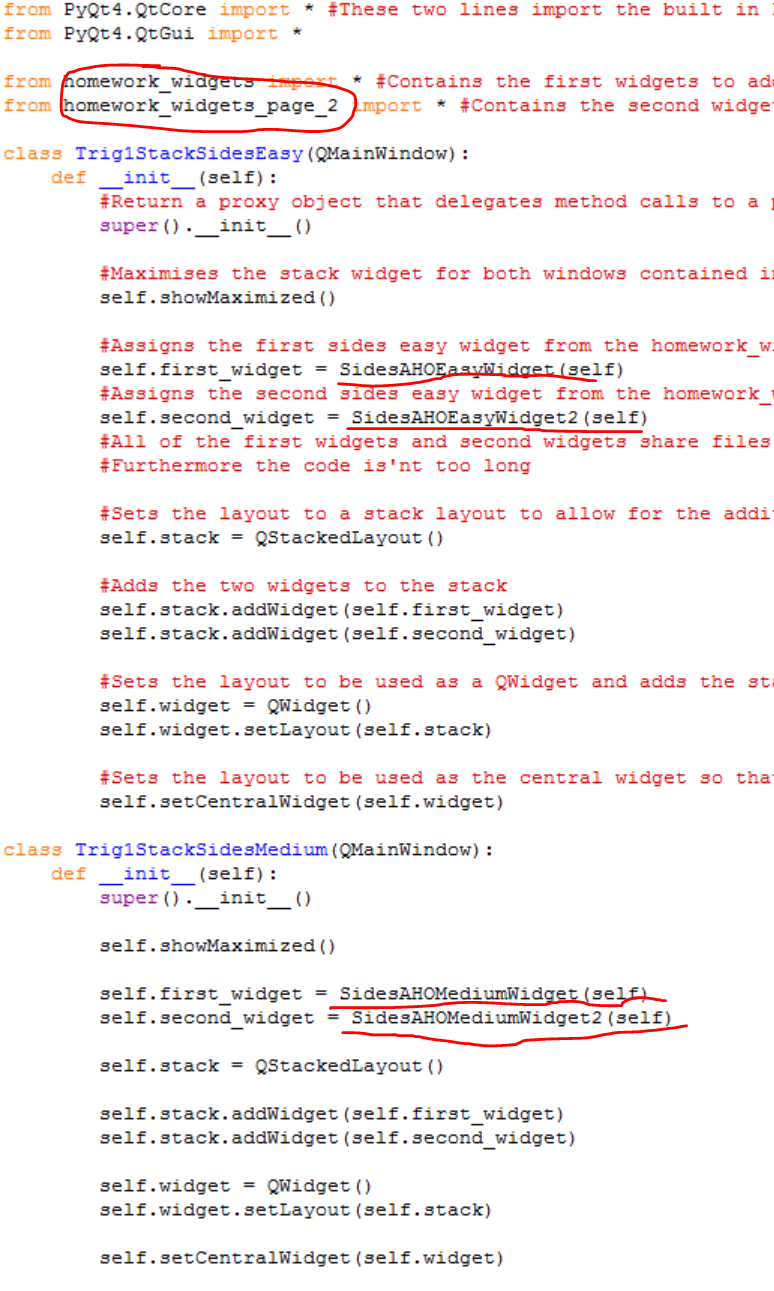
\includegraphics{C:/Users/Jordan/git/COMP4Coursework2/Evaluation/maintainability_1}
	\caption{An example of subclasses which share a file import being created in the same file with similar names}
\end{figure}

\begin{figure}[H]
	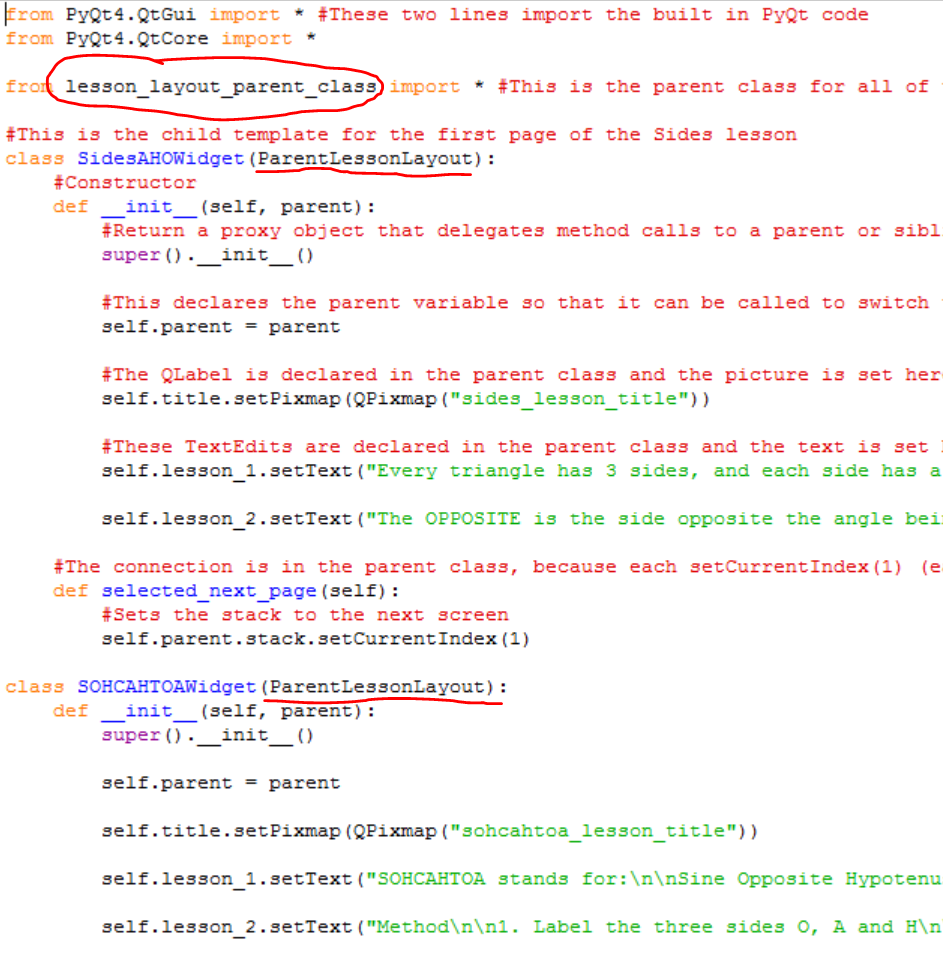
\includegraphics{C:/Users/Jordan/git/COMP4Coursework2/Evaluation/maintainability_2}
	\caption{An example of subclasses which share a parent class being created in the same file with similar names}
\end{figure}

\begin{figure}[H]
	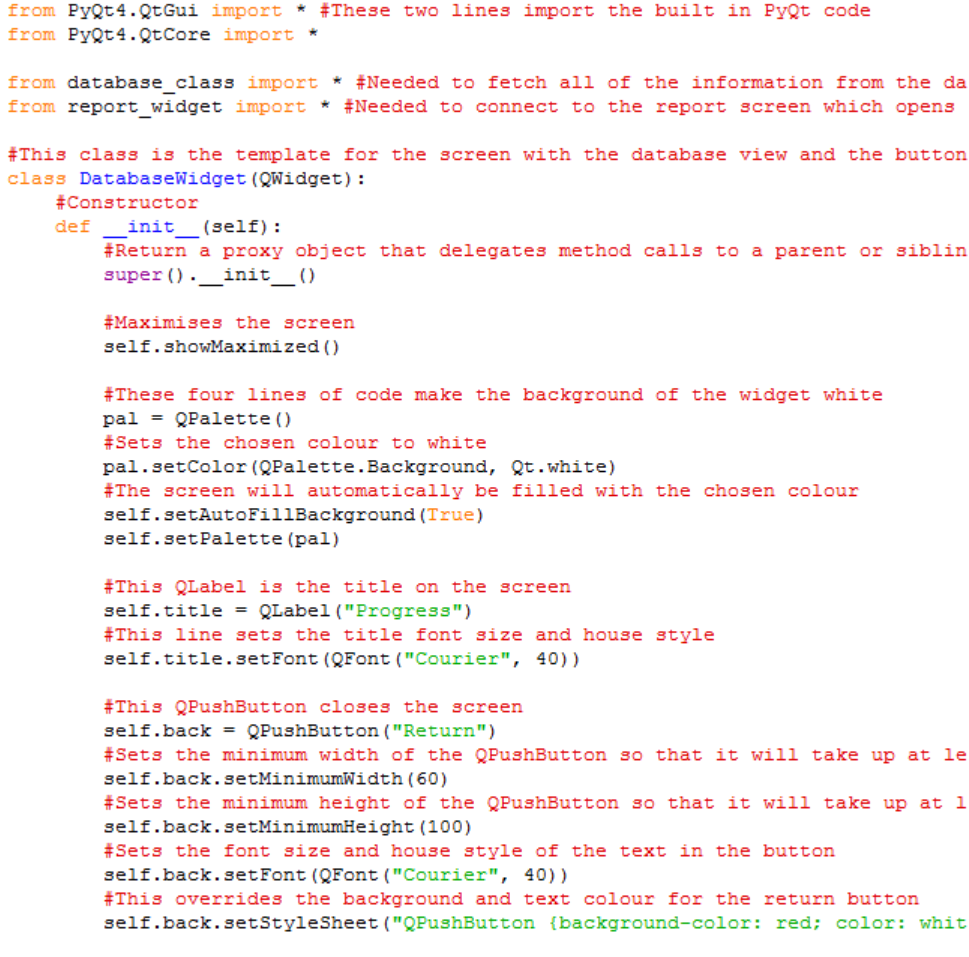
\includegraphics{C:/Users/Jordan/git/COMP4Coursework2/Evaluation/maintainability_3_1}
	\caption{This shows the structure of the code in a class, consistent in all modules}
\end{figure}

\begin{figure}[H]
	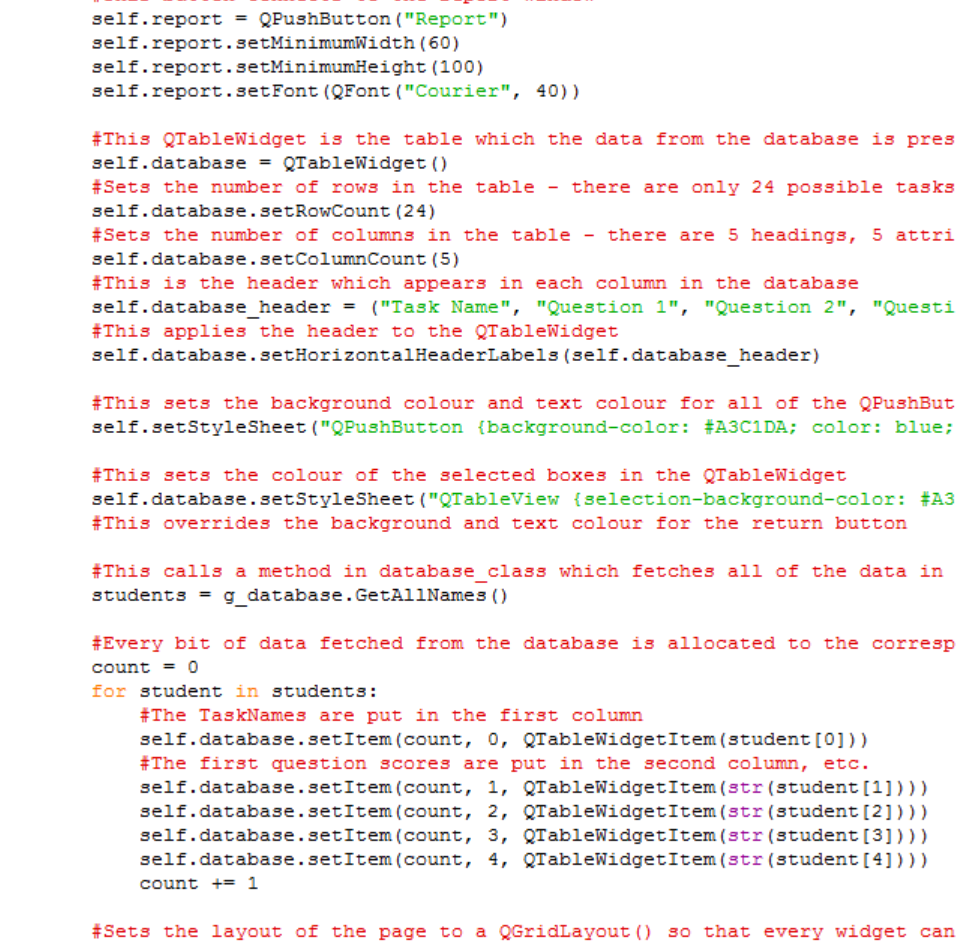
\includegraphics{C:/Users/Jordan/git/COMP4Coursework2/Evaluation/maintainability_3_2}
	\caption{This shows the structure of the code in a class, consistent in all modules}
\end{figure}

\begin{figure}[H]
	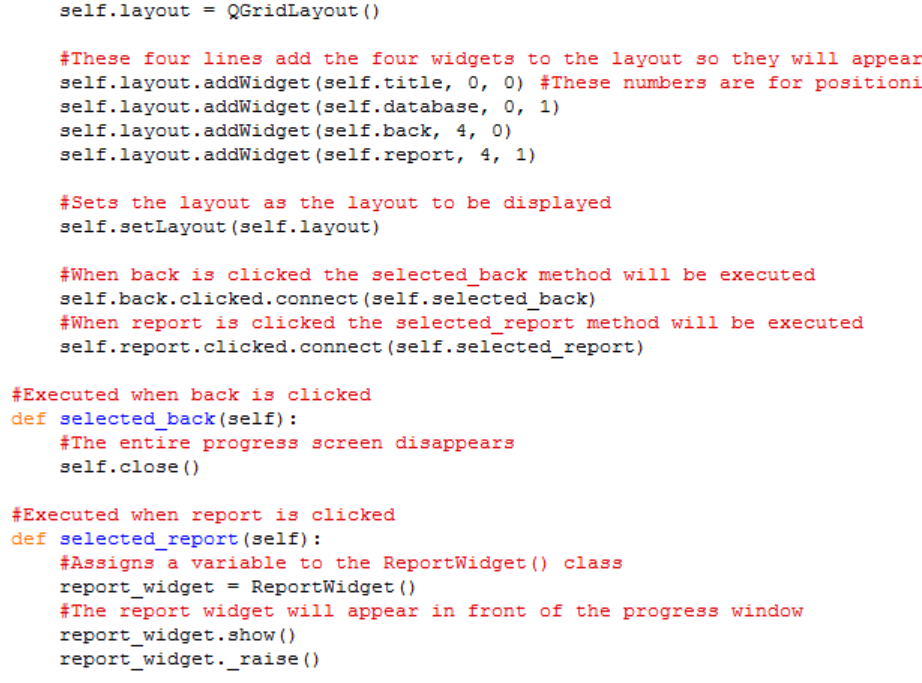
\includegraphics{C:/Users/Jordan/git/COMP4Coursework2/Evaluation/maintainability_3_3}
	\caption{This shows the structure of the code in a class, consistent in all modules}
\end{figure}

\begin{figure}[H]
	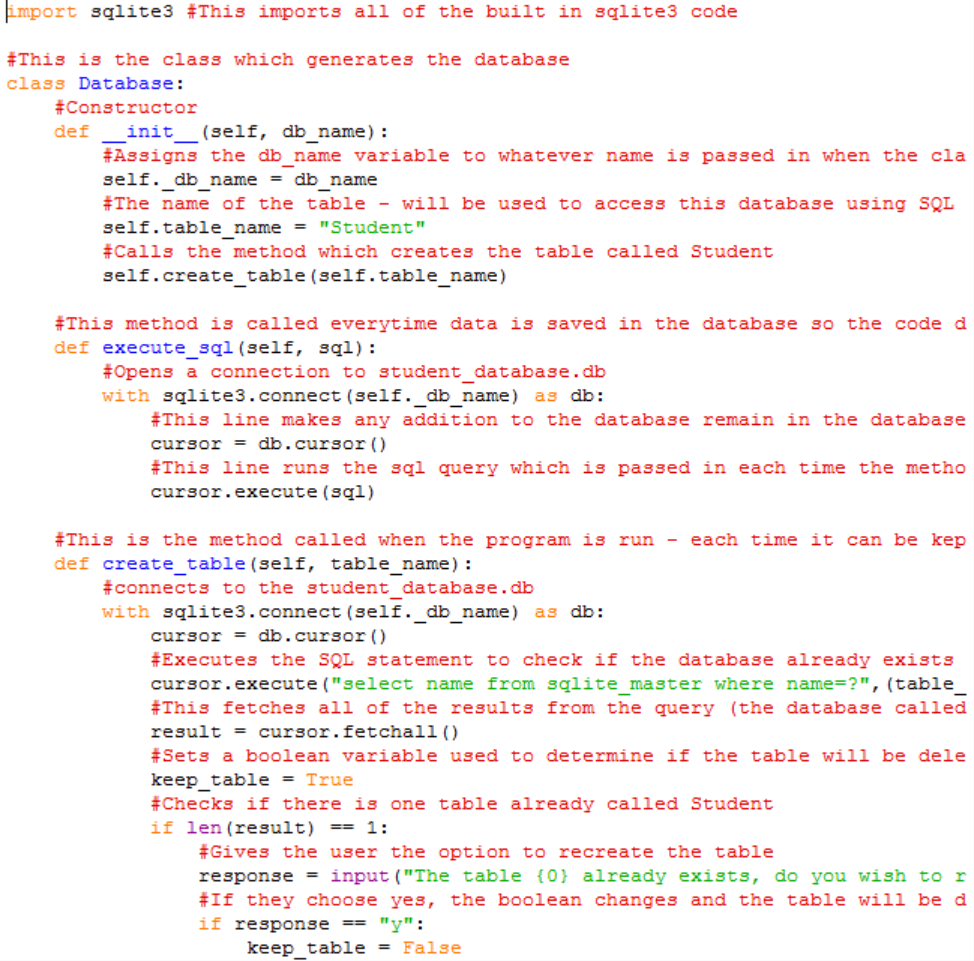
\includegraphics{C:/Users/Jordan/git/COMP4Coursework2/Evaluation/maintainability_4_1}
	\caption{This shows the database controller code all in the same class}
\end{figure}

\begin{figure}[H]
	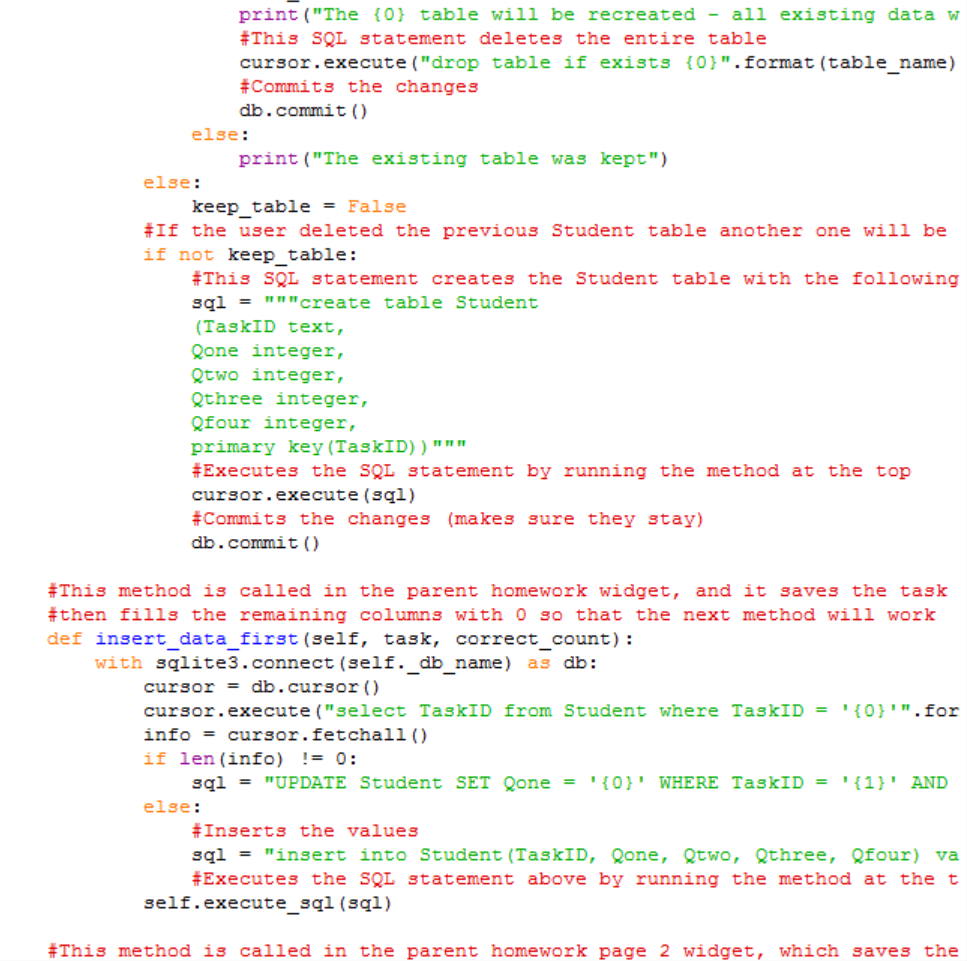
\includegraphics{C:/Users/Jordan/git/COMP4Coursework2/Evaluation/maintainability_4_2}
	\caption{This shows the database controller code all in the same class}
\end{figure}

\begin{figure}[H]
	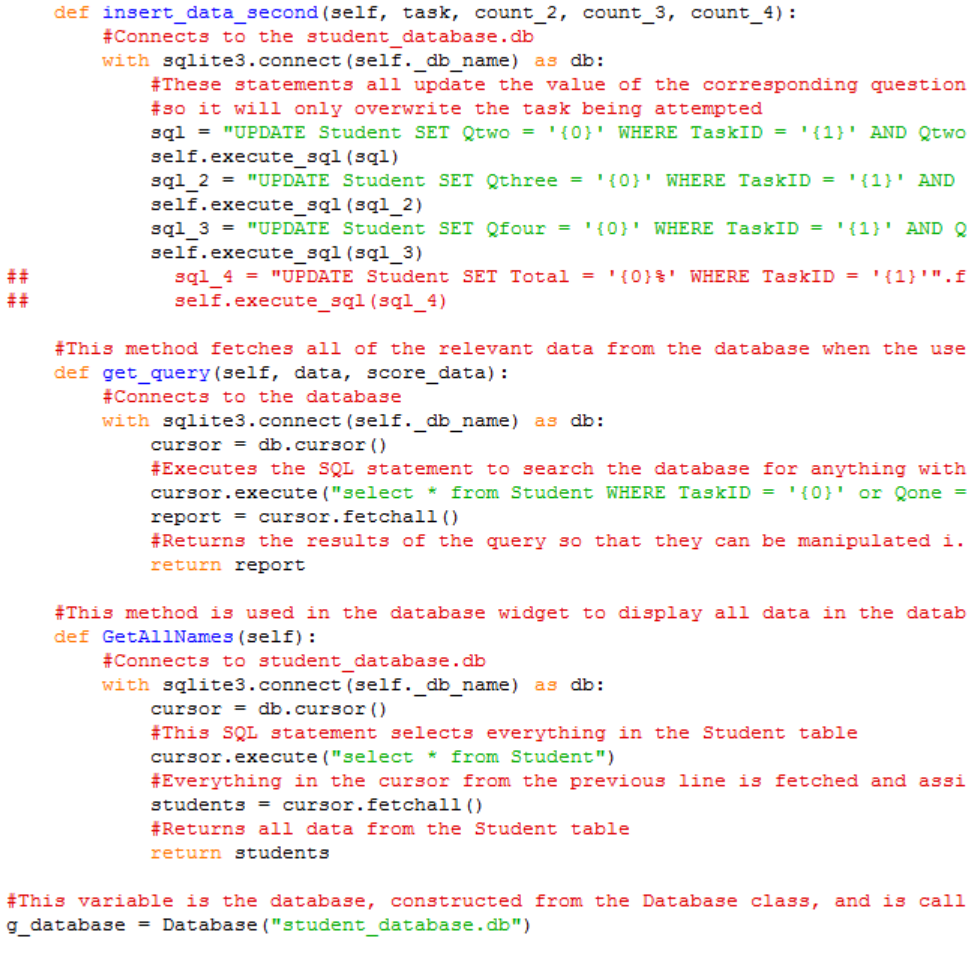
\includegraphics{C:/Users/Jordan/git/COMP4Coursework2/Evaluation/maintainability_4_3}
	\caption{This shows the database controller code all in the same class}
\end{figure}

\begin{figure}[H]
	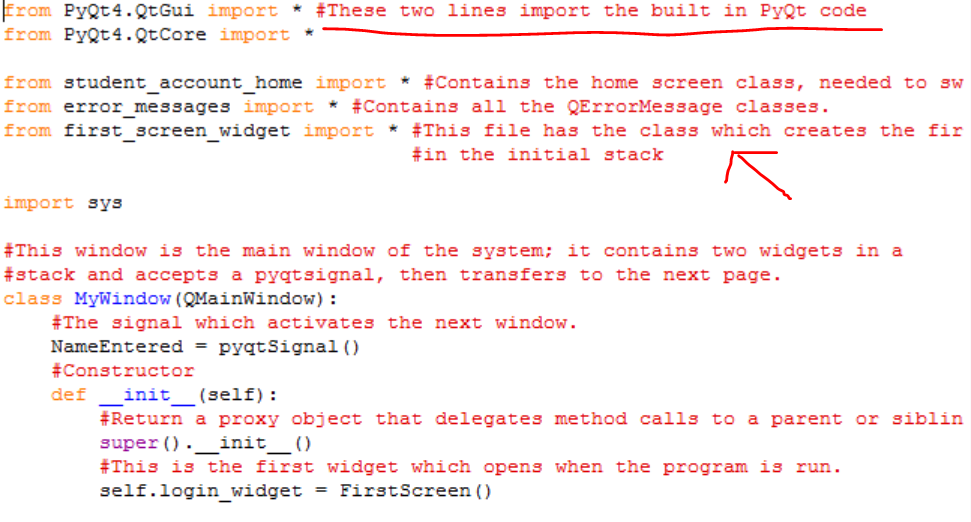
\includegraphics{C:/Users/Jordan/git/COMP4Coursework2/Evaluation/maintainability_5}
	\caption{Examples of comments used to explain the purpose of code segments}
\end{figure}

In terms of system parameters, there are none which could or should be manually changed or ever changed, as usually the parameters are passed into the database controller for database changes to be made. If the structure of the entire database were changed in a future version, then new parameters might need to be placed in the methods in the database controller class and in the places where these methods are called. Otherwise, for the current version of the system, the database can only be modified if the appropriate parameters have been obtained, such as a task score, as error messages are in place to make it impossible for a user to skip a parameter. All of the possible parameter values are hard-coded, and that need not ever be changed as it would potentially involve writing pointlessly complex code for the same purpose as the current code.

\begin{figure}[H]
	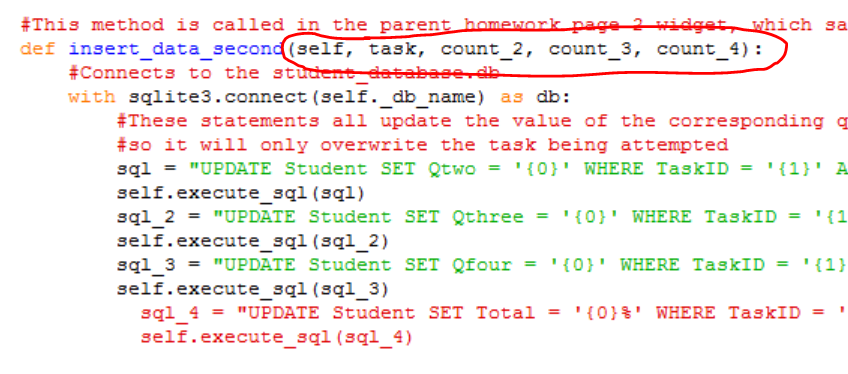
\includegraphics{C:/Users/Jordan/git/COMP4Coursework2/Evaluation/maintainability_6}
	\caption{The parameters accepted by the database controller methods}
\end{figure}

\begin{figure}[H]
	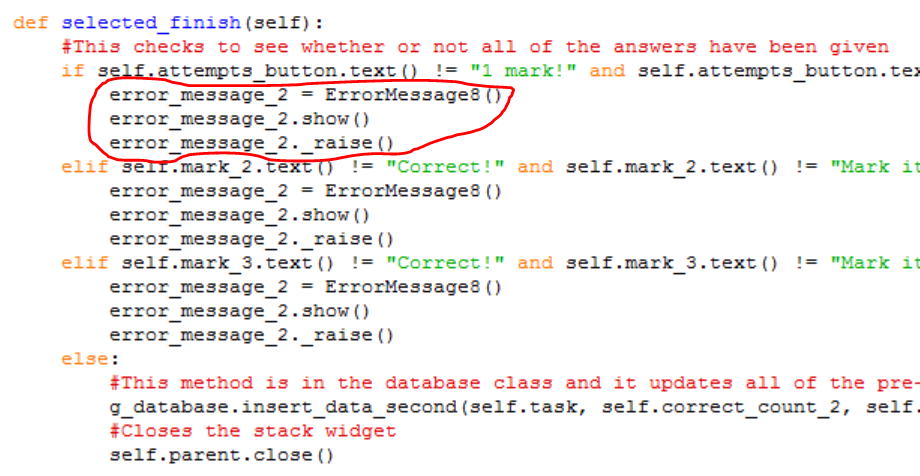
\includegraphics{C:/Users/Jordan/git/COMP4Coursework2/Evaluation/maintainability_7}
	\caption{Example of an error message used to prevent the user skipping a parameter}
\end{figure}

\begin{figure}[H]
	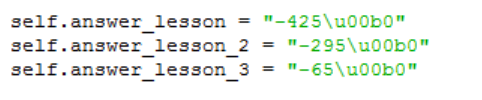
\includegraphics{C:/Users/Jordan/git/COMP4Coursework2/Evaluation/maintainability_8}
	\caption{Example of hard-coded parameters which must not be changed}
\end{figure}

On the other hand, one possible short coming relating to the system's maintainability is that, with the subclasses, they are all crammed into one file, so the programmer will have to scroll through the file to find the right subclass. Another issue is that it is not immediately clear where the file with the destination of a connection is, for example, in one file a method might be designed to open another window with a lesson, but if there was an error in that method, the programmer would have to know where the class which is being opened is in the files (i.e. the lesson page class) if the class name was wrong or something like that. 

\begin{figure}[H]
	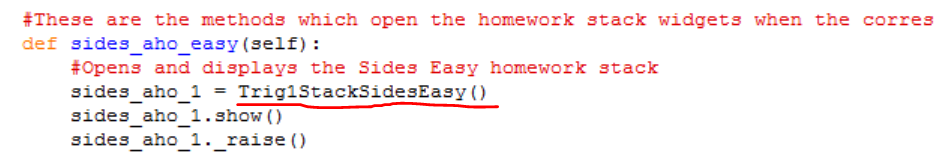
\includegraphics{C:/Users/Jordan/git/COMP4Coursework2/Evaluation/maintainability_9}
	\caption{Examples of a method where it can be unclear where the class which is being assigned to the variable is located}
\end{figure}

Overall, my code has been organised in a way which is intended to maximise maintainability by making it easier to know where a piece of code is likely to be. The classes are organised under clear file names, and relevant variable, method and class names have been used to make it clear what the purpose of a class might be, or the function of a method. It might be difficult to locate specific subclasses, but there are comments in place to make it easier in some cases, such as which file contains a parent class which subclasses are inheriting from. Finally, the system parameters all work solidly and need never be changed. Therefore, this system has a reasonably high level of maintainability.

\section{Suggestions for Improvement}

\textbf{Include Administrator Capabilities}

By far the biggest short coming from the original client objective specification, the lack of administrator capabilities prevents the client from having an effective way to ensure that students are making the required progress, resorting them to trust alone. Responsible students will be more likely to achieve more by using this system despite not being monitored by the client, but less responsible students might miss out on the boost that this system could provide them.

\textbf{Include a local area network system which can connect multiple computers with multiple user accounts}

It would be useful to have different accounts so that students can access their progress from any computer with the system installed, or at least any computer in a LAN. This way they would be able to use the system in class.

\textbf{Include more entities in the database}

The current database is useful for showing the user which aspects of the maths in the system they need to improve on, but it would be far better to have names and ratings recorded so the client could monitor the students' progress more easily.

\textbf{Include an input type that isn't just clicking or typing, such as drag and drop functionality}

There is a range of input types, but they are not necessarily that far off from one another. The system includes typing in text boxes, selecting from drop down combo boxes (multiple choice) and clicking multiple choice buttons, which all involve clicking or typing. Drag and drop functionality would provide a much wider range of input types and make the system somewhat less boring to use after a while.

\section{End User Evidence}

The following images are of a feedback form which I provided to the client so they could convey to me the extent to which they were satisfied with the system.

\begin{figure}[H]
	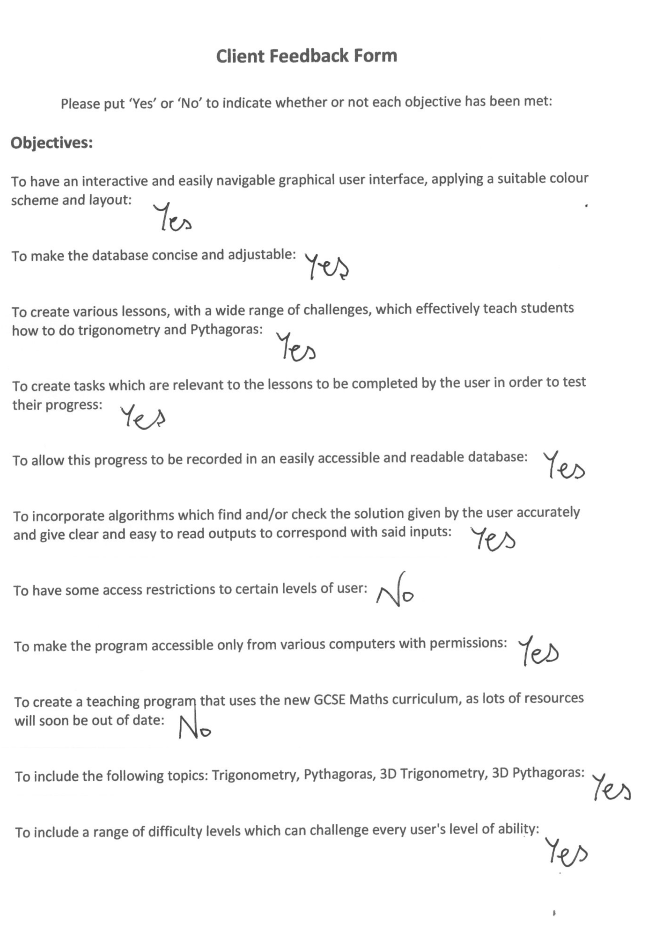
\includegraphics{C:/Users/Jordan/git/COMP4Coursework2/Evaluation/client_feedback_1}
\end{figure}

\begin{figure}[H]
	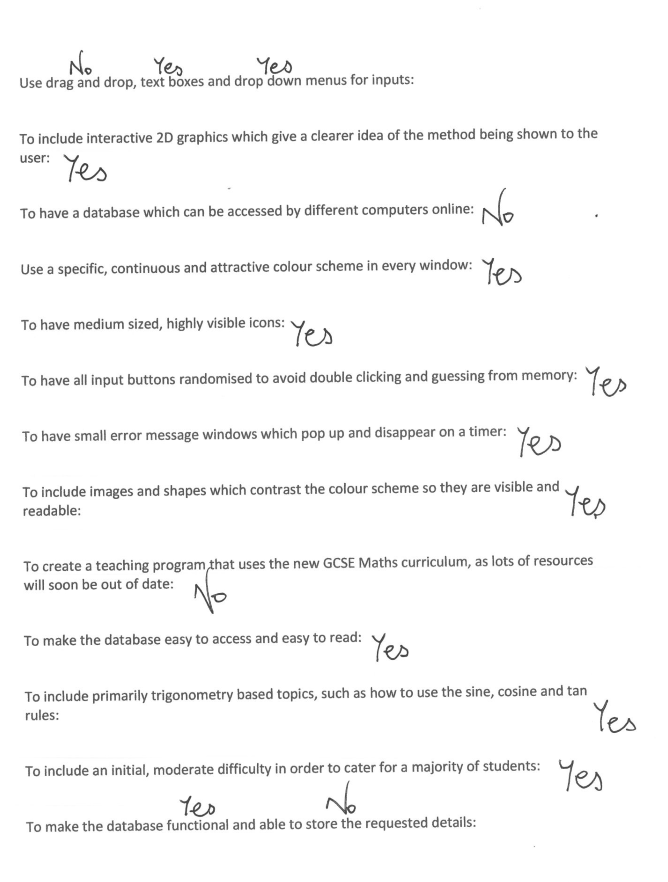
\includegraphics{C:/Users/Jordan/git/COMP4Coursework2/Evaluation/client_feedback_2}
\end{figure}

\begin{figure}[H]
	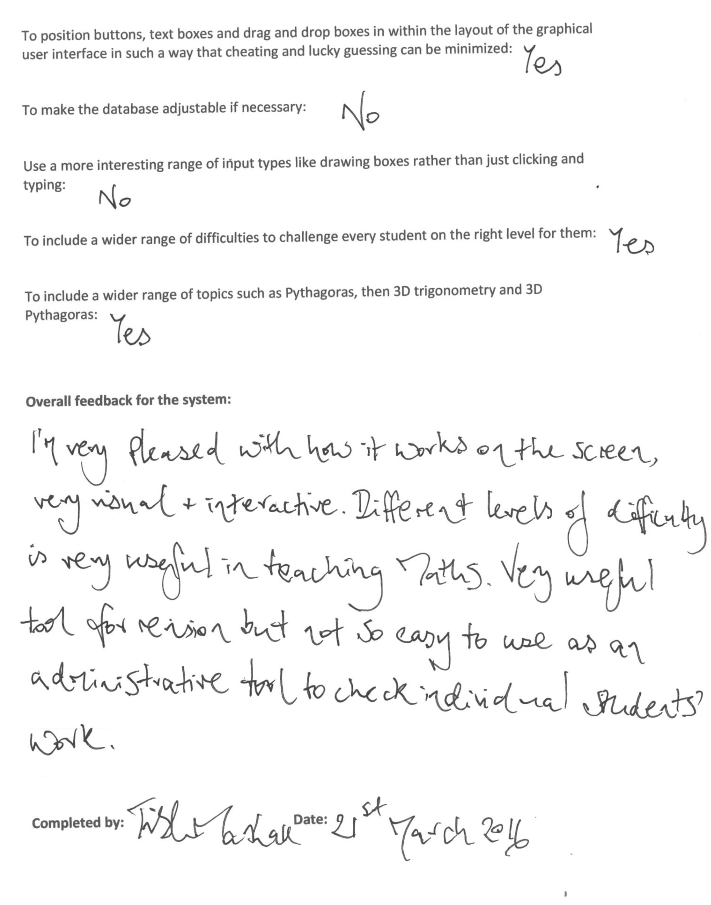
\includegraphics{C:/Users/Jordan/git/COMP4Coursework2/Evaluation/client_feedback_3}
\end{figure}

\subsection{Questionnaires}

This was a brief questionnaire given to the client to give a broad idea of how satisfied they are with the system.

\begin{figure}[H]
	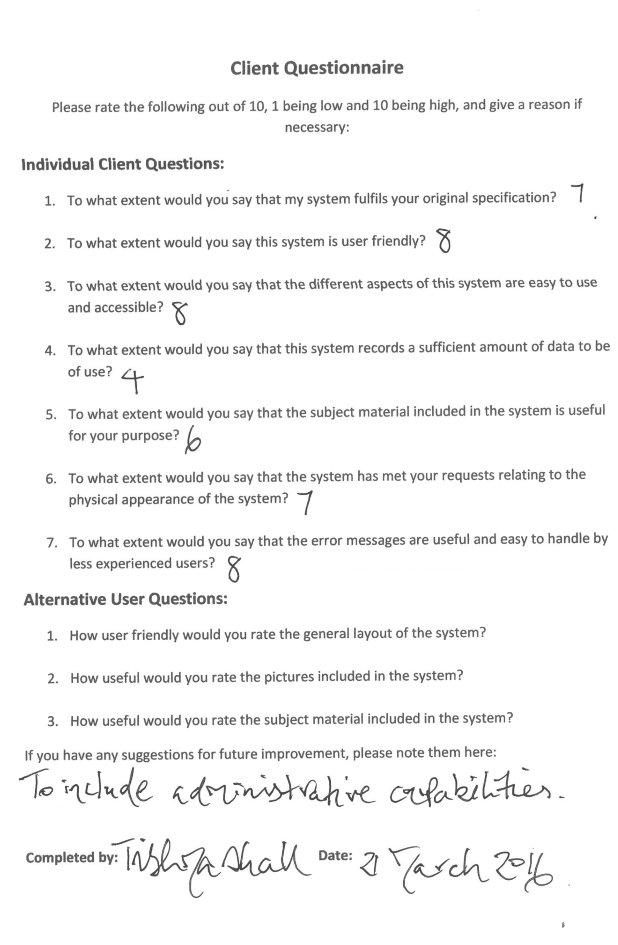
\includegraphics{C:/Users/Jordan/git/COMP4Coursework2/Evaluation/client_questionnaire}
\end{figure}

\subsection{Graphs}

This graph shows the balance of how satisfied the client is with the system:

\begin{figure}[H]
	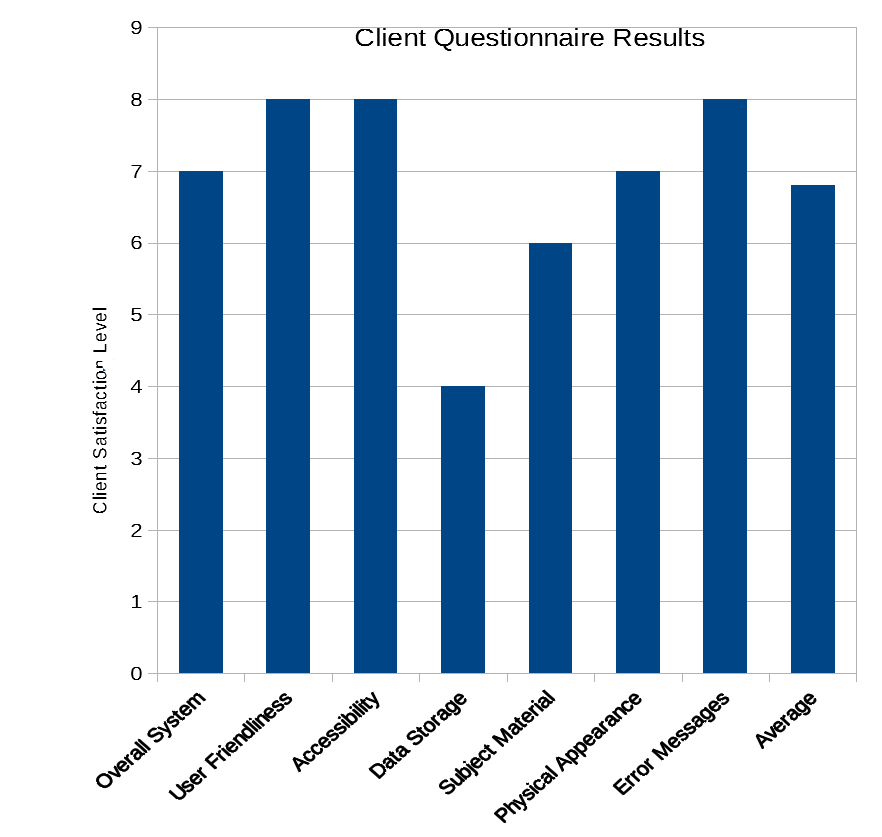
\includegraphics{C:/Users/Jordan/git/COMP4Coursework2/Evaluation/client_graph}
	\caption{According to this graph, the customer was satisfied with 68\% of the system.}
\end{figure}

This graph shows each of the client's 'yes' marks  against the number of 'no' marks related to whether or not each objective was achieved (out of 32 objectives/sub-objectives, some of which were only partially achieved):

\begin{figure}[H]
	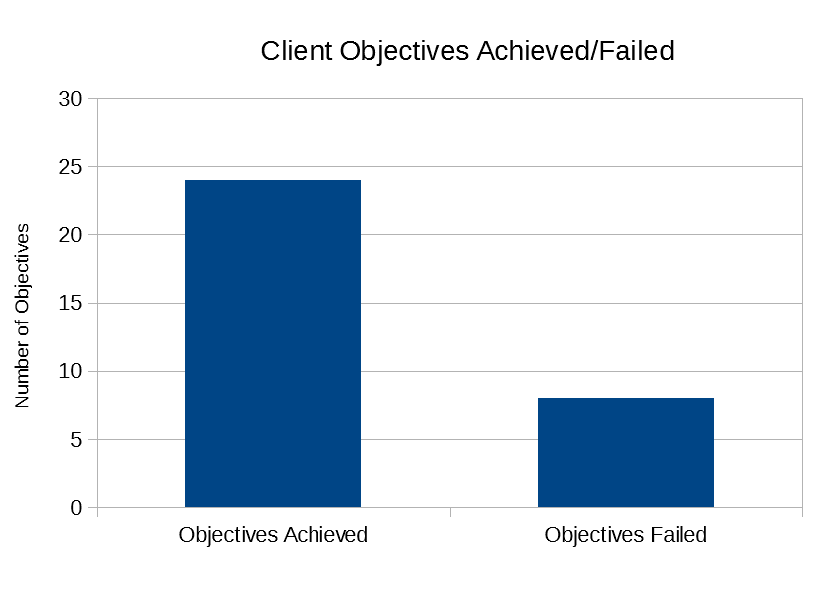
\includegraphics{C:/Users/Jordan/git/COMP4Coursework2/Evaluation/client_graph_2}
	\caption{According to this graph, the customer believed I had achieved 75\% of their specified objectives.}
\end{figure}